\section{mr::sphere\-Sampler Class Reference}
\label{classmr_1_1sphereSampler}\index{mr::sphereSampler@{mr::sphereSampler}}
Sample spherically or partially around a sphere.  


{\tt \#include $<$mr\-Sampler.h$>$}

Inheritance diagram for mr::sphere\-Sampler::\begin{figure}[H]
\begin{center}
\leavevmode
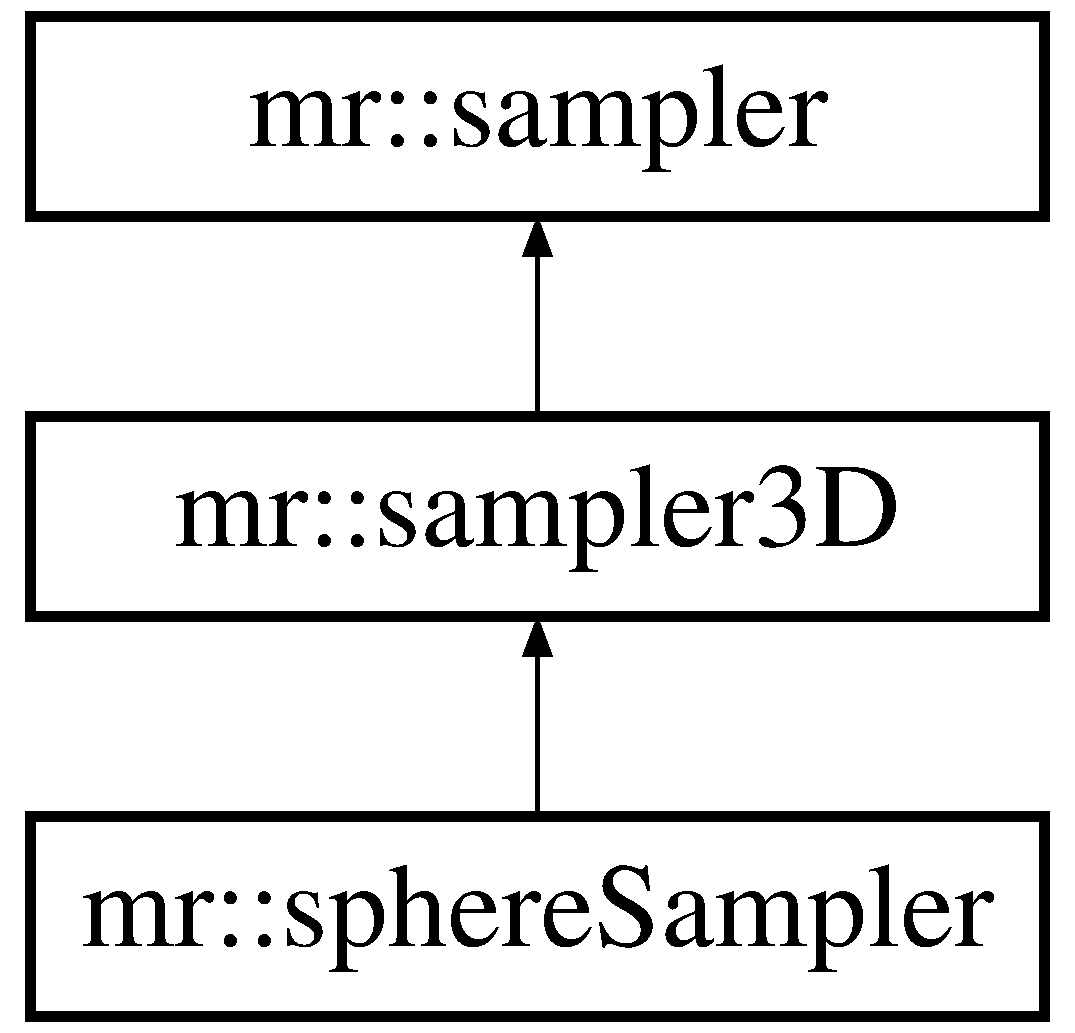
\includegraphics[height=3cm]{classmr_1_1sphereSampler}
\end{center}
\end{figure}
\subsection*{Public Member Functions}
\begin{CompactItemize}
\item 
{\bf sphere\-Sampler} (const mi\-Vector \&Nin, const mi\-Scalar sphere\-Percent=1.0f)
\item 
{\bf sphere\-Sampler} (const mi\-Vector \&Nin, const mi\-Uint \&num\-Samples, const mi\-Scalar sphere\-Percent=1.0f)
\item 
{\bf $\sim$sphere\-Sampler} ()
\begin{CompactList}\small\item\em Destructor. \item\end{CompactList}\item 
const mi\-Scalar {\bf weight} ()
\item 
bool {\bf uniform} (const mi\-State $\ast$const state)
\begin{CompactList}\small\item\em Get one sample using a uniform distribution or return false. \item\end{CompactList}\end{CompactItemize}
\subsection*{Protected Member Functions}
\begin{CompactItemize}
\item 
void {\bf calculate\-Direction} ()
\item 
void {\bf uniform\-Distribution} ()
\end{CompactItemize}


\subsection{Detailed Description}
Sample spherically or partially around a sphere. 



\subsection{Constructor \& Destructor Documentation}
\index{mr::sphereSampler@{mr::sphere\-Sampler}!sphereSampler@{sphereSampler}}
\index{sphereSampler@{sphereSampler}!mr::sphereSampler@{mr::sphere\-Sampler}}
\subsubsection{\setlength{\rightskip}{0pt plus 5cm}mr::sphere\-Sampler::sphere\-Sampler (const mi\-Vector \& {\em Nin}, const mi\-Scalar {\em sphere\-Percent} = 1.0f)\hspace{0.3cm}{\tt  [inline]}}\label{classmr_1_1sphereSampler_a0}


Constructor. Nin is the direction to sample around. sphere\-Percent is percentage of sphere to cover. If sphere percent is 1, Nin is irrelevant. This call is to be used when sampling adaptively (ie. the number of samples to be taken are not known or may vary, or you may exit the loop early). \index{mr::sphereSampler@{mr::sphere\-Sampler}!sphereSampler@{sphereSampler}}
\index{sphereSampler@{sphereSampler}!mr::sphereSampler@{mr::sphere\-Sampler}}
\subsubsection{\setlength{\rightskip}{0pt plus 5cm}mr::sphere\-Sampler::sphere\-Sampler (const mi\-Vector \& {\em Nin}, const mi\-Uint \& {\em num\-Samples}, const mi\-Scalar {\em sphere\-Percent} = 1.0f)\hspace{0.3cm}{\tt  [inline]}}\label{classmr_1_1sphereSampler_a1}


Constructor. Nin is the direction to sample around. sphere\-Percent is percentage of sphere to cover. If sphere percent is 1, Nin is irrelevant. num\-Samples is the number of samples to take. It HAS to be mi\-Uint\& \index{mr::sphereSampler@{mr::sphere\-Sampler}!~sphereSampler@{$\sim$sphereSampler}}
\index{~sphereSampler@{$\sim$sphereSampler}!mr::sphereSampler@{mr::sphere\-Sampler}}
\subsubsection{\setlength{\rightskip}{0pt plus 5cm}mr::sphere\-Sampler::$\sim${\bf sphere\-Sampler} ()\hspace{0.3cm}{\tt  [inline]}}\label{classmr_1_1sphereSampler_a2}


Destructor. 



\subsection{Member Function Documentation}
\index{mr::sphereSampler@{mr::sphere\-Sampler}!calculateDirection@{calculateDirection}}
\index{calculateDirection@{calculateDirection}!mr::sphereSampler@{mr::sphere\-Sampler}}
\subsubsection{\setlength{\rightskip}{0pt plus 5cm}void mr::sphere\-Sampler::calculate\-Direction ()\hspace{0.3cm}{\tt  [inline, protected]}}\label{classmr_1_1sphereSampler_b0}


\index{mr::sphereSampler@{mr::sphere\-Sampler}!uniform@{uniform}}
\index{uniform@{uniform}!mr::sphereSampler@{mr::sphere\-Sampler}}
\subsubsection{\setlength{\rightskip}{0pt plus 5cm}bool mr::sphere\-Sampler::uniform (const mi\-State $\ast$const {\em state})\hspace{0.3cm}{\tt  [inline]}}\label{classmr_1_1sphereSampler_a4}


Get one sample using a uniform distribution or return false. 

\index{mr::sphereSampler@{mr::sphere\-Sampler}!uniformDistribution@{uniformDistribution}}
\index{uniformDistribution@{uniformDistribution}!mr::sphereSampler@{mr::sphere\-Sampler}}
\subsubsection{\setlength{\rightskip}{0pt plus 5cm}void mr::sphere\-Sampler::uniform\-Distribution ()\hspace{0.3cm}{\tt  [inline, protected]}}\label{classmr_1_1sphereSampler_b1}


\index{mr::sphereSampler@{mr::sphere\-Sampler}!weight@{weight}}
\index{weight@{weight}!mr::sphereSampler@{mr::sphere\-Sampler}}
\subsubsection{\setlength{\rightskip}{0pt plus 5cm}const mi\-Scalar mr::sphere\-Sampler::weight ()\hspace{0.3cm}{\tt  [inline]}}\label{classmr_1_1sphereSampler_a3}


This returns a weight (dot product) of the sample with respect to the original Nin vector. 

The documentation for this class was generated from the following file:\begin{CompactItemize}
\item 
{\bf mr\-Sampler.h}\end{CompactItemize}
